\section{Tackling Problem 2}
\label{sec:problem-2}

\begin{figure*}[t]
    \centering
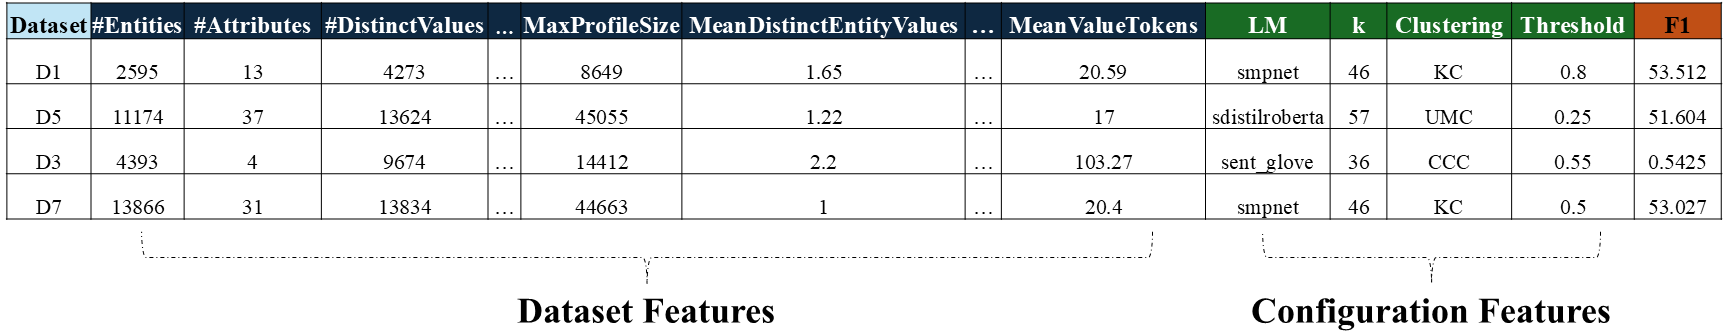
\includegraphics[width=0.95\linewidth]{figures/dataset/join_dataset_trials.png}
    \caption{The feature vector of the regression model addressing Problem \ref{pr:pr2}. It combines 12 dataset features with 4 configuration parameters of the ETEER pipeline in Figure \ref{fig:eeter_pipeline}. Note that the leftmost column ("Dataset") is only added for clarification  purposes.}
    \label{fig:join_dataset_trials}
\end{figure*}

To address Problem \ref{pr:pr2}, we define a regression model that treats every combination of a dataset $D$ and a set of configuration values $V$ as an instance. For the labelled instances, the dependent variable corresponds to the F1 score of the ETEER pipeline in Figure \ref{fig:eeter_pipeline}, configured with $V$, when applied on $D$. For the unlabelled instances, the goal is to predict this F1 score. 

To put this approach into practice, we need to define the following aspects of the regression model:

\begin{itemize}[leftmargin=*]
    \item Feature engineering. This means that we need to define the feature vector that is fed to the regression model during the training and prediction phases. This vector consists of two types of dimensions: (i) \textit{dataset features}, and (ii) \textit{configuration features}. For the former, which capture the characteristics of a Record Linkage dataset, we consider features from dataset profiles defined in the literature, as explained in Section \ref{sec:datasetProfiling}. For the configuration features, the definition is straightforward: there is a separate feature for each parameter of the ETEER pipeline in Table \ref{tab:parameter-values}. The domain of each feature is the same as the respective numeric parameter, in the case of $k$ and the similarity threshold. The categorical parameters (i.e., LM and clustering algorithm) are transformed into a binary format through one-hot encoding. 
    \item Instance generation. We define three approaches for generating the labelled instances that will be used for training the regression model: (i) grid search, (ii) sampling-based search, and (iii) their combination. The resulting configuration features are combined with the dataset features extracted from the datasets D1-D10 in Table \ref{tab:dataset-specs} except for the one that should be fine-tuned. For each feature vector, we apply the respective parameter configuration to a particular dataset with known ground truth in order to estimate the corresponding target variable, i.e., the F1-score. 
    \item Learning process. We use two methods for training the regression model: (i) Random Forest and (ii) AutoML. A critical characteristic is that both methods incorporate feature selection, which is necessary due to the high dimensionality of the feature vector defined by feature engineering and the unclear contribution of each dimension. Another crucial characteristic is that they both achieve very high performance under versatile settings \cite{DBLP:journals/csur/KarmakerHSXZV22,DBLP:journals/bioinformatics/NguyenJGSALJCGM21}.
\end{itemize}

%{\color{red}As explained above, the sampling algorithms are guided by the performance that corresponds to each tested configuration. In the context of Problem 2, though, this approach is inapplicable, due to the lack of a ground truth for the dataset at hand. Nevertheless, ETEER fine-tuning can still be modelled as a learning-based task by leveraging the ground truths from other datasets.

%When no ground truth file is provided, a pyJedAI user does not have the ability to use the methodology described earlier \comments{[why?]}. Also, configurations must be data sensitive, meaning that we need to extract some generic features from the given dataset. \comments{explain more the features extracted?}
%\comments{Here, we describe what we CANNOT do, but we should describe also what we actually do.}

%\begin{table}[t]
{\footnotesize
\begin{center}  
\label{tab:featureSet}
\begin{tabular}{|p{2cm}|p{5cm}|}\hline
\textbf{Dataset Feature} & \textbf{Definition} \\
\hline
Number of entities & The total number of entities in the dataset \\ \hline
Number of attributes & The total number of attributes for the entities \\ \hline
Number of distinct values & The total number of distinct values across all attributes \\ \hline
Number of name-value pairs & The total number of name-value pairs in the dataset \\ \hline
Mean name-value pairs per entity & The average number of name-value pairs per entity \\ \hline
Mean name-value pairs per attribute & The average number of name-value pairs per attribute \\ \hline
Number of missing name-value pairs & The total number of missing name-value pairs in the dataset \\ \hline
Mean distinct values per attribute & The average number of distinct values per attribute \\ \hline
Mean total attribute value length per entity & The average total length of attribute values per entity \\ \hline
Mean attribute value tokens per entity & The average number of tokens in attribute values per entity \\ \hline
Mean distinct values per entity & The average number of distinct values per entity \\ \hline
Max values per entity & The maximum number of values for any single entity \\ \hline
\end{tabular}
\caption{The list of dataset features.}
\end{center}  
}
\end{table}

%\subsection{Building a model over trials}

%The previous experimental methodology involved multiple runs of different executions on ten distinct datasets \comments{what datasets?}, resulting in a comprehensive trials dataset. In this new approach, the trials and configurations serve as our primary data. 
%More specifically, we frame our solution to Problem 2 as a regression task that is addressed in the following way: 
%\begin{enumerate}[leftmargin=*]
%    \item Dataset profiling: We define a set of features that capture the characteristics of a Record Linkage dataset.
%    \item Definition of independent variables: The \textit{dataset features} defined in the previous step are concatenated with four \textit{configuration features}, which stand for the four configuration parameters of the ETEER pipeline in Figure \ref{fig:eeter_pipeline}. This means that each feature vector combines parameter configurations with general characteristics of a particular dataset.
%    \item Estimation of dependent variables: For each feature vector, we apply the respective parameter configuration to a particular dataset with known ground truth in order to estimate the corresponding target variable, i.e., the corresponding F1-score. Applying numerous ETEER configurations to multiple datasets with known ground truth yields a sizeable training set.
%    \item Model training: A regression algorithm is trained on the labelled instances generated by the previous steps.
%    \item Prediction phase: The learned model is applied to the feature vectors extracted from the given dataset $D$ through grid search. Note that there is a different feature vector for each parameter configuration we want to try, while dataset $D$ lacks any ground truth. The feature vector yielding the highest predicted F1-score 
    %(\comments{mipws F1-score opws to exeis sto section 2?}) 
    %is selected as the optimal configuration for dataset $D$.
%\end{enumerate}
%To put this idea into practice, we need to implement the following:
%\begin{enumerate}[leftmargin=*]
%    \item Dataset Profiling: define the dataset features capturing general characteristics of an ER dataset,
%    \item Instance Generation: define the approach for generating the configuration values to be tested.
%\item Choose the datasets with known ground truth that will generate the training instances.
%    \item Learning process: define the method used for training a performance prediction model.
%\end{enumerate}
%For Point (3), we choose a set of 11 established datasets for Record Linkage that are publicly available and widely used in the literature, while encompassing a complete ground truth. See Section \ref{sec:experiments} for more details. We delve into Points (1), (2) and (4) in the following.
%}

We delve into each of these three steps in the following.

\subsection{Feature Engineering}
\label{sec:datasetProfiling}

The dataset features used by our approach should adhere to the following principles: 
\begin{enumerate}[leftmargin=*]
    \item They should be \textit{generic}, applying seamlessly to any ER dataset, regardless of its format (i.e., be it structured like a CSV file or semi-structured like JSON file or RDF dump) and regardless of the corresponding flavor of ER (i.e., Record Linkage, Deduplication or Multi-source ER).
    \item They should be \textit{effective}, capturing all aspects of given dataset $D$ that might affect the performance of an ETEER pipeline on~$D$.
    \item They should be \textit{efficient}, involving low extraction cost and overhead, so that it is possible to extract predictions for numerous feature vectors from the learned model.
\end{enumerate}

In this context, we consider the following wide range of dataset features, which captures the main ones proposed in the literature. Our goal is to perform feature selection during the learning process so as to identify the top performing features for the task at hand.
\begin{enumerate}[leftmargin=*, label=F\arabic*), start=1]
    \item \#Entities \cite{DBLP:conf/sigmod/IlyasMHBA04}: the total number of entities in the dataset, i.e., $|\mathcal{E}_1| + |\mathcal{E}_2|$ in the case of Record Linkage datasets. This feature 
    %is an indication of the size of the dataset, which 
    affects proportionately the number of nearest neighbors returned for each query entity.
    \item \#Attributes: The total number of distinct attributes describing all given entities in $\mathcal{E}_1$ and $\mathcal{E}_2$. This is an indication of the schema heterogeneity of the given dataset(s), with higher values indicating more heterogeneous and noisy datasets. This is called schema complexity in~\cite{DBLP:conf/cikm/PrimpeliB20}.
    \item \#DistinctValues \cite{DBLP:conf/sigmod/IlyasMHBA04}: the total number of distinct values across all attributes. Higher values suggest a larger diversity in the description of entity profiles, which indicates more challenging settings for an ETEER pipeline.
    \item \#AttributeValuePairs: the total number of attribute-value pairs in all entity profiles of the given dataset(s). Higher values indicate larger profile sizes, which are probably harder to match.
    \item MeanProfileSize: the average number of attribute-value pairs per entity, i.e., F4/F1. The rationale is the same as~F4.
    %\comments{mipws attribute-value pairs? epeidi sto 2 kai 3 les attributes}
    \item MeanAttributeSize: the average number of name-value pairs per attribute, i.e., F4/F2. Higher values indicate attributes with a larger domain, thus diversifying the entity descriptions and rendering ER a more challenging~task.
    \item MeanDistinctEntityValues: the average number of distinct values per entity, i.e., F3/F1. Lower values indicate profiles with insufficient or repeated information, thus hampering ER.
    \item MeanDistinctAttributeValues~\cite{DBLP:journals/pvldb/SuchanekAS11}: the average number of distinct values per attribute, i.e., F3/F2. Low values indicate datasets with non-distinctive attribute-value pairs, which are thus harder to deduplicate.
    \item MaxProfileSize: the maximum number of attribute-value pairs in any of the given entities. Higher values indicate harder entity matching settings, e.g., datasets with oversized profiles, which are probably associated with irrelevant and, thus, noisy values. 
    \item MissingInformation: The total number of missing attribute-value pairs in the given dataset(s), which is estimated as F1 $\times$ F7 - F4. Higher values indicate higher levels of noise in the given datasets, which hamper ER. This is called sparsity in~\cite{DBLP:conf/cikm/PrimpeliB20}.
    \item MeanValueTokens: The average number of tokens in all attribute values per entity. Lower values correspond to datasets with small entity descriptions, which probably lack sufficient information for ER. This is called textuality in~\cite{DBLP:conf/cikm/PrimpeliB20}.
    \item MeanValueLength: This is a variation of MeanValueTokens (or textuality \cite{DBLP:conf/cikm/PrimpeliB20}). It concatenates all attribute values per entity in a sentence, but instead of counting the words formed by tokenizing it on whitespace, it measures its length in characters. This length is averaged, across all input entities. Longer values indicate richer entity profiles, which might involve more distinguishing information, facilitating their deduplication.
\end{enumerate}

Note that all dataset features satisfy the requirements defined above, being generic, effective and efficient. They are concatenated with the four configuration features of the ETEER pipeline in Figure~\ref{fig:eeter_pipeline}, forming the 16-dimensional feature vector in Figure~\ref{fig:join_dataset_trials}.


\subsection{Instance Generation}
\label{sec:instanceGeneration}

%given a dataset, we extract a set of features and predict the optimal configuration. This is achieved by training a model based on configuration values and dataset features, with the goal of predicting the F1 score. The top-1 configuration, which has the maximum predicted F1 score, is then proposed as the optimal configuration. Three different approaches \comments{[which are..?]} were tested to ensure the best results and model generalization. 

We follow three different procedures for generating a set of labelled instances from every dataset:
\begin{enumerate}[leftmargin=*]
    \item \textit{Grid search} applies all configurations in Table \ref{tab:parameter-values} to estimate the dependent variable per instance, i.e., the respective F1-score.
    \item \textit{Sampling-based search} applies the four sampling methods in Section \ref{sec:problem-1} for a specific number of trials. F1-score is only estimated for these trials, yielding an equal number of labelled instances.
    \item \textit{All} merges the instances generated by the two approaches.
    %grid and sampling-based search.
\end{enumerate}

%Grid search is expected to yield a larger number of instances than sampling-based search, because the latter is bounded by the limited budget of trials. 
In all cases, we exclude instances with a zero F1 as well as duplicate instances, which have the same configuration (e.g., proposed by different samplers).
%rials, where samplers proposed configurations already covered by the grid search, were also removed from the training sets. 
Note that instance generation is a time-consuming process, due to the large number of ETEER pipelines that are evaluated. However, it constitutes an offline process that is carried out only once and, thus, does not affect the prediction time when applying the trained regression model on a new dataset that lacks a ground truth.
%for our approach when it is applied to a new dataset. %{\color{red}Nevertheless, we experimentally evaluate not only the effectiveness but also the time efficiency of this step in Section \ref{sec:expProblem2}. ISWS TO VGALOUME AUTO. DEN KSERW AN EXEI NOIMA. VASILIS: SYMFWNW


%Among these methods, grid search is expected to involve a much more time-consuming process, due to the larger number of configurations that it typically considers. However, the actual run-time of the configurations tested by grid search might be much lower than that of the configurations proposed by sampling-based search. Most importantly, instance generation is an offline process that does not affect the prediction time for the learned model. Therefore, we are mostly interested in the effectiveness of the models learned by each instance generation approach. This is experimentally assessed in Section \ref{sec:experiments}. 

\subsection{Learning process}
\label{sec:learningProcess}

%\begin{table}[ht]
\centering
\caption{Parameters Tested for RF Regression Method.}
\label{tab:regressor_params}
\begin{tabular}{|p{1.5cm}|l|l|}
\hline
\textbf{Regressor}          & \textbf{Parameter}        & \textbf{Search Space}                           \\ \hline
% \multirow{1}{*}{Lasso}      & alpha                     & \text{LogUniform}($10^{-4}$, $10^1$)                           \\ \hline
% \multirow{1}{*}{Ridge}      & alpha                     & \text{LogUniform}($10^{-4}$, $10^1$)                           \\ \hline
% \multirow{1}{*}{LR} & -                 & -                                               \\ \hline
% \multirow{8}{*}{XGBR} & n\_estimators    & $\{100,...,1000\} \subseteq \mathbb{Z}$                                   \\ \cline{2-3}
%                             & max\_depth                 & $\{3,...,10\} \subseteq \mathbb{Z}$                                      \\ \cline{2-3}
%                             & learning\_rate             & \text{LogUniform}($10^{-3}$, $10^{-1}$)                          \\ \cline{2-3}
%                             & subsample                 & \text{Uniform}($0.5$, $1.0$)                                                \\ \cline{2-3}
%                             & colsample\_bytree          & \text{Uniform}($0.5$, $1.0$)                               \\ \cline{2-3}
%                             & gamma                     & $\{0,...,5\} \subseteq \mathbb{Z}$                                        \\ \cline{2-3}
%                             & reg\_alpha                 & \text{LogUniform}($10^{-2}$, $10^{2}$)                              \\ \cline{2-3}
%                             & reg\_lambda                & \text{LogUniform}($10^{-2}$, $10^{2}$)                              \\ \hline
\multirow{5}{*}{RFR} & n\_estimators & $\{100, ..., 1000\} \subseteq \mathbb{Z}$                                  \\ \cline{2-3}
                            & max\_depth                 &  $\{3,...,10\} \subseteq \mathbb{Z}$                                      \\ \cline{2-3}
                            & min\_samples\_split         &  $\{2,...,20\} \subseteq \mathbb{Z}$                                      \\ \cline{2-3}
                            & min\_samples\_leaf          &  $\{1,...,20\} \subseteq \mathbb{Z}$                                      \\ \cline{2-3}
                            & max\_features              & $\{ sqrt, log2\}$                            \\ \hline
% \multirow{3}{*}{NN}         & hidden\_dim                &  $\{16,...,128\} \subseteq \mathbb{Z}$                                    \\ \cline{2-3}
%                             & lr                         & \text{LogUniform}($10^{-5}, 10^{-2}$)                          \\ \cline{2-3}
%                             & num\_epochs                &  $\{2,...,50\} \subseteq \mathbb{Z}$                                      \\ \hline
\end{tabular}
\end{table}


%So far, we described the process for assembling a large set of labelled instances that associate the dataset and configuration features with the corresponding \comments{F1-score}. This process is applied to datasets D1-D10 described in Section \ref{sec:expSetup} except for the dataset is given as input to be fine-tuned (in a vein similar to leave-one-out cross-validation). For this dataset, we feed all feature vectors to the trained to retrieve the predicted F1-score per configuration. %To train the prediction model, we consider two learning approaches: 
Having generated labelled instances from datasets with known ground truth, we train a regression model that estimates the F1-score per feature vector (i.e., per pipeline configuration and dataset without ground truth), in two different ways:
\begin{enumerate}[leftmargin=*]
    \item Random Forest (RF) \cite{DBLP:conf/icdar/Ho95}. This a simple, yet effective, approach to learn an ensemble of regression models. RF contains five hyperparameters whose tuning is essential: n\_estimators $\in \{100, ..., 1000\} \subseteq \mathbb{Z}$,  max\_depth  $ \in \{3,...,10\} \subseteq \mathbb{Z}$, min\_samples\_split $\in \{2,...,20\} \subseteq \mathbb{Z}$, min\_samples\_leaf $\in \{1,...,20\} \subseteq \mathbb{Z}$, max\_features $\in \{ sqrt, log2\}$.
    To fine-tune within these domains, we leverage Optuna as follows: First, we split the labelled instances into train and validation sets, with the latter created in a stratified manner so that it contains 10\% of the instances from each known dataset. Next, Optuna uses the validation set to find a near-optimal parameter set within 50 trials, by minimizing the mean squared error. 
    %MSE on the validation set. Five key hyperparameters (n) are optimized. Each hyperparameter is explored within predefined intervals, as outlined in the Appendix.
    %\sout{Linear Regression (LR). It constitutes the simplest solution to the regression task of estimating the F1 per instance. Its main advantages are: (i) its high time efficiency, given that both the training and the prediction process have a rather low overhead, and (ii) its parameter-free functionality, which waives the need for hyperparameter estimation.}
    \item AutoML \cite{DBLP:journals/kbs/HeZC21}. 
    %Instead of manually testing several state-of-the-art regression algorithms, 
    This approach evaluates a wide range of ML algorithms, such as decision trees and neural networks, without any human intervention. It also performs automatic hyperparameter optimization, considering models and configurations that might be overlooked during a manual process. For this reason, it typically yields higher accuracy than any manual procedure.
    %{\color{red}WHY DID WE OPTED FOR AUTOML? WHAT ARE THE ADVANTAGES? HOW DOES IT WORK?
    %CAN WE FOCUS AUTOML ON LEARNING ALGORITHMS WITH INTEGRATED FEATURE SELECTION?}
    %\item \textit{Individual regressors.} The following regression algorithms were considered:  Linear Regression, Lasso, Ridge, Random Forest Regressor, Gradient Boosting (XGBoost) Regressor as well as a Neural Network (NN). The neural network, defined using PyTorch, is designed with adjustable parameters including the size of the hidden layer, learning rate, and number of epochs. Optuna (\comments{8eloume ref sto optuna?}) conducts a series of trials (50 in our setup) to identify the optimal hyperparameters that minimize the validation loss. The neural network architecture consists of an input layer, one hidden layer with ReLU activation and dropout for regularization, and an output layer. The Adam optimizer is used for training, and a learning rate scheduler adjusts the learning rate based on the validation loss. Early stopping is implemented to halt training when the validation loss no longer improves, ensuring the model does not overfit. Hyperparameter optimization is performed using the TPESampler algorithm, which efficiently explored the configuration space we defined for each algorithm.
    %for each regressor to identify the optimal hyperparameters,
    %In fact, the fine-tuning minimized the mean squared error on a validation set derived from 10\% of a stratified random sample from the training data. After determining the best hyperparameters, the model is retrained on the full training set and used to predict the F1-scores of the test set. This process is applied independently to each dataset. The only exception is Linear Regression, which is a parameter-free approach.
\end{enumerate}

Note that both RF and AutoML learn train regression models on subsets of the features of Section~\ref{sec:datasetProfiling}. That is, both inherently apply \textit{feature selection}. The main difference is that RF assigns the same weight to each individual model, taking the average of their predictions, whereas AutoML considers a weighted arithmetic mean. In more detail,
%At this point, it is worth elaborating on the latter. AutoML relies on 
%Based on \cite{DBLP:conf/icml/CaruanaNCK04}, 
AutoML first explores and optimizes different regression models and then uses their predictions on the validation set 
%from these models 
to build an ensemble from the top N performing models \cite{DBLP:conf/icml/CaruanaNCK04} -- in our case, N goes up to 5. In fact, 
%Based on each model's , 
a weight is assigned to each model in proportion to its performance on the validation set, so that better-performing models receive greater weights. To make its final predictions, AutoML computes a weighted average of the predictions from the individual models.
%In other words,\textit{ LR learns a linear combination of the features in Section \ref{sec:datasetProfiling}, while AutoML learns a linear combination of models trained on the features of Section~\ref{sec:datasetProfiling}}.